\subsection{Neighborhood Search Strategy}
\label{subsec:neighborhood-search-strategy}

Despite its straightforward implementation, this method presents significant computational challenges. For a grid comprising \(n \times n\) points, the process involves solving \(n^2\) subproblems, each requiring \(\mathcal{O}(n^2)\) operations. This leads to a total computational complexity of \(\mathcal{O}(n^4)\), making the method computationally intensive, especially for large-scale applications.

To mitigate these computational demands, a strategic limitation of the search area for each subproblem is proposed, as illustrated in Figure \ref{fig:dyn-prog-full-disc-search}. The size of this area must be adaptable based on the grid's dimensions; a fixed size may excessively restrict path movement in smaller grids. Employing this neighborhood search strategy significantly reduces computational cost to \(\mathcal{O}(n^2 |\mathcal{N}(n)|)\), where \(|\mathcal{N}(n)|\) indicates the search area's size.

\begin{figure}
    \centering
    \begin{subfigure}{.3\textwidth}
        \centering
        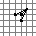
\includegraphics[width=\linewidth]{figures/dyn-prog-full-disc-search-2/fig.pdf}
        \caption{}
        \label{fig:dyn-prog-full-disc-search-2}
    \end{subfigure}%
    \begin{subfigure}{.3\textwidth}
        \centering
        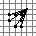
\includegraphics[width=\linewidth]{figures/dyn-prog-full-disc-search-3/fig.pdf}
        \caption{}
        \label{fig:dyn-prog-full-disc-search-3}
    \end{subfigure}%
    \begin{subfigure}{.3\textwidth}
        \centering
        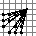
\includegraphics[width=\linewidth]{figures/dyn-prog-full-disc-search-4/fig.pdf}
        \caption{}
        \label{fig:dyn-prog-full-disc-search-4}
    \end{subfigure}
    \caption[Search Areas for Fully Discretized Reparameterization]{Visualization of limited search areas for different values of search depth \(m\): (a) \(m = 2\), (b) \(m = 3\), and (c) \(m = 4\). These figures demonstrate how increasing search depths expand the area being considered, thereby influencing the computational cost and efficiency of the reparameterization process.}    
    \label{fig:dyn-prog-full-disc-search}
\end{figure}

The limited search area is defined as follows:
\begin{equation}
    \mathcal{N}_{(i, j)}(n) = \{(k, l) \mid i-m \leq k < i, \, j-m < l < j, \, \gcd(i - k, j - l) = 1\},
    \label{eq:search-area}
\end{equation}
where \(m = f(n) \in \mathbb{N}^+\) is a function of the grid size \(n\) that determines the extent of the search area. The condition \(\gcd(i - k, j - l) = 1\) ensures that the path does not traverse any intermediate grid points, maintaining a direct route between the specified points and improving the computational efficiency of the process.

To illustrate the implementation of this strategy, we present the pseudocode for the optimal reparameterization process using dynamic programming in Algorithm \ref{alg:optimal-reparam-dp}. This algorithm aligns two curves by optimizing the parameterizations of the second curve, reducing the computational complexity through the limited search area defined earlier.

\begin{algorithm}
    \caption{Optimal Reparameterization via Dynamic Programming}
    \label{alg:optimal-reparam-dp}
    \begin{algorithmic}[1]
    \Require $c_1, c_2$: Curves, $I_1, I_2 \in \mathbb{R}$: Initial parameterizations
    \Function{OptimizeReparam}{$c_1, c_2, I_1, I_2$}
        \State $(I, c_1', c_2') \gets \text{AlignCurves}(c_1, c_2, I_1, I_2)$
        \State $(c_{1,e}', c_{2,e}') \gets \text{MoveStartToIdentity}(c_1', c_2')$ \Comment{\eqref{eq:maurer-cartan-gl}}
        \State $(q_1, q_2) \gets \text{vee}(\text{SRVT}(c_{1,e}', c_{2,e}'))$ \Comment{\eqref{eq:srvt-discrete}, \eqref{eq:vee_SO3}, \eqref{eq:vee_SE3}}
        \State $A, P \gets \text{ComputeCostMatrix}(q_1, q_2)$  \Comment{\eqref{eq:cost-matrix}}
        \State $\text{path} \gets \text{TraceOptimalPath}(P)$ 
        \State $I_{2, opt} \gets \text{LinearInterpolate}(\text{path}_x, \text{path}_y)(I_2)$ 
        \State $c_{2, opt} \gets \text{Interpolate}(I_{2}, I_{2, opt})(c_2)$  \Comment{\eqref{eq:interpolation-discrete}}
        \State \Return $(c_{2, opt}, I_{2, opt})$
    \EndFunction
    \end{algorithmic}
\end{algorithm}

The algorithm detailed in Algorithm \ref{alg:calculate-cost-parent} calculates the cost and parent matrices used in the dynamic programming approach. By leveraging the limited search area, it ensures efficient computation of the optimal path.

\begin{algorithm}
    \caption{Calculate Cost and Parent Matrices for Dynamic Programming}
    \label{alg:calculate-cost-parent}
    \begin{algorithmic}[1]
    \Require $I \in \mathbb{R}^n$: Grid points
    \Require $q_0, q_1 \in \mathbb{R}^{n-1}$: Values defined on the domain of $I$
    \Require $\text{depth} \in \mathbb{N}^+$: Depth of the search area
    \Function{calculateCostMatrixAndParent}{$I, q_0, q_1, \text{depth}$}
        \State $n \gets \text{length}(I)$
        \State $A \gets \text{matrix\_of\_infinity}(n, n)$ \Comment{Initialize cost matrix to a large value}
        \State $P \gets \text{empty matrix}(n, n)$ \Comment{Initialize parent matrix}
        
        \State $A[0, 0] \gets 0$ \Comment{Set initial cost to zero}
        \State $P[0, 0] \gets \text{None}$ \Comment{No predecessor for initial condition}
        
        \For{$i \gets 0$ \textbf{to} $n-1$}
            \For{$j \gets 0$ \textbf{to} $n-1$}
                \State $\text{preds} \gets \text{findPreds}(i, j, \text{depth})$ \Comment{\eqref{eq:search-area}}
                \For{$\text{pred} \in \text{preds}$}
                    \State $\text{cost\_to\_pred} \gets \text{localCost}(i, j, \text{pred}, q_0, q_1)$ 
                    \Comment{\eqref{eq:local-cost-functional}, \eqref{eq:local-cost-functional-SE3}}
                    \State $\text{cost} \gets \text{cost\_to\_pred} + A[\text{pred}]$ \Comment{\eqref{eq:cost-matrix}}
                    \If{$\text{cost} < A[i, j]}$
                        \State $A[i, j] \gets \text{cost}$
                        \State $P[i, j] \gets \text{pred}$
                    \EndIf
                \EndFor
            \EndFor
        \EndFor
    
        \State \Return $P, A$
    \EndFunction
    \end{algorithmic}
\end{algorithm}